%%
% Copyright (C) 2013 Dima Chumak <chumakd@gmail.com>
%
% Licensed under CC BY
% Creative Commons Attribution 3.0 License
% http://creativecommons.org/licenses/by/3.0/
%%

% warn about obsolete packages and commands (mentioned in l2tabu)
\RequirePackage[l2tabu, orthodox]{nag}

% improves the definitions of the Computer Modern font families
\RequirePackage{fix-cm}

% 'svgnames' option will be passed to xcolor, we need it if we use pdflatex,
% for latex we need 'dvipsnames' instead
%
% 'compress' -  make all navigation bars as small as possible
\documentclass[14pt,svgnames,compress]{beamer}

%
% config Beamer
%

\mode<presentation>

%\usetheme{Pittsburgh}
%\usetheme[hideothersubsections]{Hannover}
%\usetheme{Warsaw}
%\usetheme{keynote-portfolio}
\usetheme{keynote-black}

% disable subsection names in header's miniframe
%\useoutertheme[subsection=false]{smoothbars}

\newcommand{\titlefontsize}{\fontsize{64}{70}\selectfont}

\setbeamercovered{transparent}
\setbeamerfont{title}{size=\titlefontsize}

%
% include packages
%

% 'xcolor' and 'hyperref' packages are loaded by beamer,
% so no need to load it directlys

\usepackage{fixltx2e}       % fixes for latex2e which are not integrated into
                            % the kernel

\usepackage{polyglossia}    % a babel replacement for xelatex, to facilitate
                            % multilingual typesetting

\usepackage{subfigure}      % place two figures side-by-side
\usepackage{multicol}       % multi-column formatting
\usepackage{graphicx}       % enhanced version of \includegraphics command
%\usepackage{listings}       % create source code listing
\usepackage{fancyvrb}       % sofisticated verbatim output
\usepackage{tabularx}       % enhanced version of tabular environment
\usepackage{colortbl}       % colorize tables
\usepackage{setspace}       % change line spacing

\usepackage{microtype}      % use micro-typographic extensions (character
                            % protrusion font and expansion) to enhance document
                            % looking
\usepackage{tikz}           % graphics and drawings

%
% package configuration
%

%%% polyglossia %%%

% beamer uses Sans family as it's default font, so to change default font of all
% slides we should use \setsansfont command instead of \setmainfont
\setsansfont{Ubuntu}
\setmonofont{DejaVu Sans Mono}

%\setmainfont{Verdana}
%\setsansfont{Fontin Sans}
%\setsansfont{Diavlo}

%\setmainfont{CMU Serif}
%\setsansfont{CMU Sans Serif}
%\setmonofont{CMU Typewriter Text}
%\setmainfont{cmm}

\defaultfontfeatures{Scale=MatchLowercase, Mapping=tex-text}
\setdefaultlanguage{english}
\setotherlanguage[spelling=modern]{russian}

%%% hyperref %%%

%\hypersetup{colorlinks,urlcolor=SkyBlue,linkcolor=SkyBlue}
\hypersetup{colorlinks,urlcolor=SkyBlue,linkcolor=white}


%
% colors definition
%

%\definecolor{LogoColor}{RGB}{48,86,146}
\colorlet{UrlColor}{SkyBlue}
\colorlet{HlColor}{Yellow!70}


%
% custom style commands
%

%\newcommand\tablerowcolor{\rowcolor[gray]{.90}}
%\newcommand\tablecolcolor{\columncolor[gray]{.90}}
\newcommand\hl[1]{\textcolor{HlColor}{#1}}
\newcommand\frametitlefontsize{\Huge}
\newcommand\framesubtitlefontsize{\huge}

\newcommand\singleframetitle[1]{
    \begin{center}
        \frametitlefontsize #1
    \end{center}
}

\newcommand\singleframesubtitle[1]{
    \begin{center}
        \framesubtitlefontsize #1
    \end{center}
}

\newcommand\titleframe{
    \begin{frame}
        \singleframetitle{\insertsectionhead}
    \end{frame}
}

\newcommand\subtitleframe{
    \begin{frame}
        \singleframesubtitle{\insertsubsectionhead}
    \end{frame}
}

\newcommand\wordspacing[2]{
    \spaceskip=#1\fontdimen2\font plus #1\fontdimen3\font minus #1\fontdimen4\font
    #2
    \spaceskip=\fontdimen2\font plus \fontdimen3\font minus \fontdimen4\font
}

\newenvironment{wspacing}[1]
{
    \spaceskip=#1\fontdimen2\font plus #1\fontdimen3\font minus #1\fontdimen4\font
}
{
    \spaceskip=\fontdimen2\font plus \fontdimen3\font minus \fontdimen4\font
}


%
% body of presentation
%

\title{\Large{The Power of} \\ \titlefontsize\textbf{V!M}}
%\subtitle{}
\author{
    \\
    \vspace{.4cm}
    \footnotesize by \\
    \medskip  Dima Chumak \\
    chumakd@gmail.com
}
%\institute{}
\date{\footnotesize\today}


\begin{document}

\begin{frame}
    \titlepage
\end{frame}

\begin{frame}[plain]
    \begin{center}
        
\includegraphics{figures/success_vim.jpg}
    \end{center}
\end{frame}


\section{Documentation}

\begin{frame}
    \frametitle{Links}
    \begin{itemize}
        \item \href{http://www.vim.org}
                   {vim.org} - main site: docs, plugin search
        \item \href{http://vim.wikia.com}
                   {vim.wikia.com} - vim tips collection
        \item \href{http://ru.wikibooks.org/wiki/Vim}
                   {ru.wikibooks.org/wiki/Vim}
        \item \href{http://vimcasts.org/episodes/archive}
                   {vimcasts.org} - collection of video tutorials
        \item \href{http://vim-scripts.org}
                   {vim-scripts.org} - all vim plugins under git
        \item \href{http://rayninfo.co.uk/vimtips.html}
                   {rayninfo.co.uk/vimtips.html} \\
                   Best of Vim Tips by David~Rayner {\footnotesize
                   a.k.a.}~zzapper, {\footnotesize 15 years with Vim and still
                   learning ;)}
        \item \href{http://www.derekwyatt.org/vim/vim-tutorial-videos/}
                   {derekwyatt.org/vim/vim-tutorial-videos} \\
                   Derek~Wyatt's Vim video totorial
    \end{itemize}
\end{frame}

\begin{frame}[fragile]
    \frametitle{Documentation}
    \vspace{1cm}
    \Large
    :help help-context \\ \bigskip
    :help :h           \\ \bigskip
    :help              \\ \bigskip
    \verb|$ vimtutor|  \\
    \begin{center}
        \href{http://vimdoc.sourceforge.net/htmldoc}
             {vimdoc.sf.net/htmldoc}
    \end{center}
\end{frame}


\section{Core functionality}

\titleframe

\begin{frame}[plain]
    \begin{tikzpicture}[remember picture,overlay]
        \node[at=(current page.center)] {
            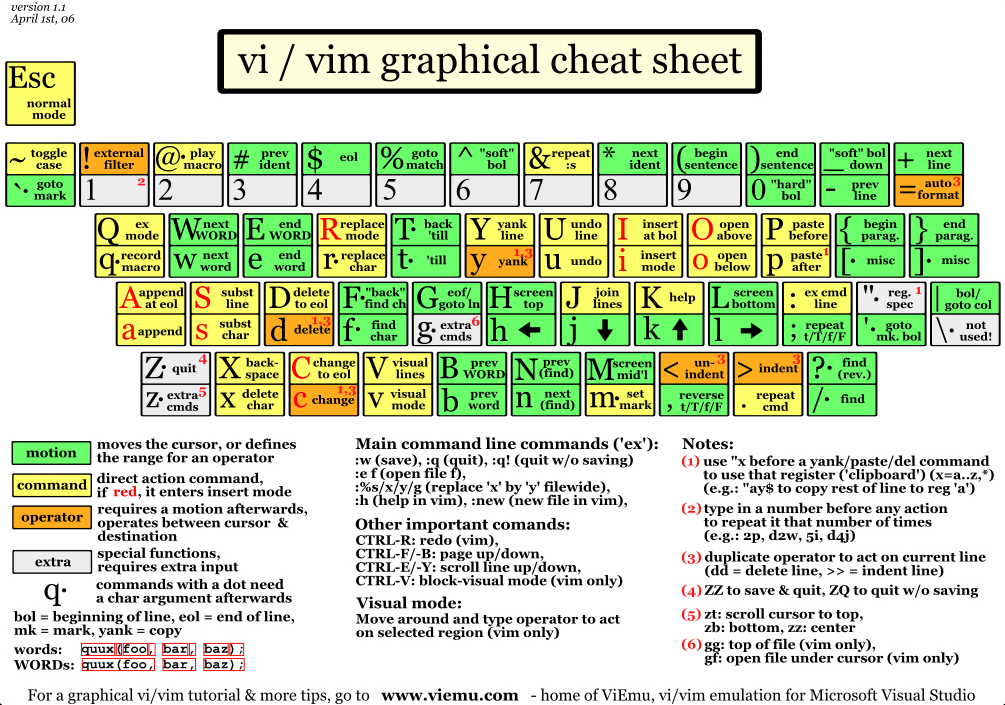
\includegraphics[width=\paperwidth]{figures/vim_cheat_sheet_cropped.jpg}
        };
    \end{tikzpicture}
\end{frame}


\subsection{Modes}

\subtitleframe

\begin{frame}[fragile]
    \begin{spacing}{1.5} % line spacing
        \Large
        \centering
        \verb|i  I  gi  a  A  o  O| \\
        \verb|R  gh  gH  v_Ctrl-g| \\
        \verb|v  V  Ctrl-v| \\
    \end{spacing}
\end{frame}


\subsection{Motion commands}

\subtitleframe

\begin{frame}
    \begin{center}
        
\includegraphics[scale=1.5]{figures/cursor_motions.jpg}
    \end{center}
\end{frame}

\begin{frame}[fragile]
    \begin{spacing}{1.5} % line spacing
        \Large
        \centering
        \verb|h  j  k  l  H  M  L (  )  {  }| \\
        \verb|w  W  b  B  e  E  ge  gE| \\
        \verb|0  $  ^  g_  g0  g$  gj  gk| \\
        \verb+f  F  t  T  ;  ,  |  gm+ \\
        \verb|/  ?  *  #  g*  g#  n  N  | \\
        \verb|gg  G  `  '  [  ]  %|
    \end{spacing}
\end{frame}


\subsection{Change operators}

\subtitleframe

\begin{frame}[fragile]
    \begin{spacing}{1.5} % line spacing
        \Large
        \centering
        \verb|c  d  y| \\
        \verb|~  g~  gu  gU| \\
        \verb|!  =  <  >| \\
        \verb|gq  gw| \\
        \verb|g?|
    \end{spacing}
\end{frame}


\subsection{Change commands}

\subtitleframe

\begin{frame}[fragile]
    \begin{spacing}{1.5} % line spacing
        \Large
        \centering
        \verb|r  R| \\
        \verb|dl  x  D  dd| \\
        \verb|Y  yy  p  P  [p  [P| \\
        \verb|s  S  C  cc| \\
        \verb|J| \\
    \end{spacing}
\end{frame}

\subsection{Text objects}

\subtitleframe

\begin{frame}[fragile]
    \begin{spacing}{1.5} % line spacing
        \Large
        \centering
        \verb|iw  iW  aw  aW| \\
        \verb|is  as     ip  ap     it  at| \\
        \verb|ib  ab  i(  a(  i)  a)| \\
        \verb|iB  aB  i{  a{  i}  a}| \\
        \verb|i<  a<  i>  a>| \\
        \verb|i"  i'  i`  a"  a'  a`|
    \end{spacing}
\end{frame}


\subsection{Undo/Redo}

\subtitleframe

\begin{frame}[fragile]
    \begin{spacing}{1.5} % line spacing
        \Large
        \centering
        \verb|u  Ctrl-r| \\ \bigskip
        \verb|U  g+  g-|
    \end{spacing}
    % TODO: ref Gundo plugin
\end{frame}


\subsection{Text completion}

\subtitleframe

\begin{frame}[fragile]
    \begin{spacing}{1.5} % line spacing
        \begin{columns}
            \column{0.5\textwidth}
                \centering
                i\_Ctrl-x\_Ctrl-\hl{l} \\
                i\_Ctrl-x\_Ctrl-\hl{n} \\
                i\_Ctrl-x\_Ctrl-\hl{k} \\
                i\_Ctrl-x\_Ctrl-\hl{t} \\
                i\_Ctrl-x\_Ctrl-\hl{i} \\
                i\_Ctrl-x\_Ctrl-\hl{]} \\
            \column{0.5\textwidth}
                \centering
                i\_Ctrl-x\_Ctrl-\hl{f} \\
                i\_Ctrl-x\_Ctrl-\hl{d} \\
                i\_Ctrl-x\_Ctrl-\hl{v} \\
                i\_Ctrl-x\_Ctrl-\hl{u} \\
                i\_Ctrl-x\_Ctrl-\hl{o} \\
                i\_Ctrl-x\_\hl{s}~~~~i\_Ctrl-\hl{n} \\
        \end{columns}
    \end{spacing}
\end{frame}


\subsection{Macros}

\subtitleframe

\begin{frame}[fragile]
    \begin{spacing}{1.5} % line spacing
        \Large
        \centering
        \verb|q|\hl{\{0-9a-zA-Z"\}} \\
        \verb|q| \\
        \verb|@|\hl{\{0-9a-z".=*\}} \\
        \verb|@@| \\
    \end{spacing}
\end{frame}


\subsection{Search/Replace}

\subtitleframe

\begin{frame}[fragile]
    \begin{spacing}{1.5} % line spacing
        \Large
        \centering
        \verb|/  ?  n  N| \\ \bigskip
        \verb|*  g*  #  g#| \\
        \vspace{1cm}
        \normalsize
        :\hl{s}/XXX/YYY/\hl{flags} \\
        \verb|&  g&| \\
        :\hl{g}/XXX/\hl{command} \\
    \end{spacing}
\end{frame}


\subsection{Scrolling}

\subtitleframe

\begin{frame}[fragile]
    \begin{spacing}{1.5} % line spacing
        \Large
        \centering
        \verb|Ctrl-f  Ctrl-b| \\
        \verb|Ctrl-d  Ctrl-u| \\
        \verb|Ctrl-e  Ctrl-y| \\ \bigskip
        \verb|zt  zz  zb| \\
        \verb|zl  zh  zL  zH| \\
    \end{spacing}
\end{frame}


\subsection{Buffers}

\subtitleframe

\begin{frame}[fragile]
    \begin{spacing}{1.5} % line spacing
        \Large
        \centering
        \verb|:ls  :b|\hl{N} \\ \bigskip
        \verb|:bufdo| \\ \bigskip
        \verb|Ctrl-^| \\
    \end{spacing}
\end{frame}


\subsection{Windows}

\subtitleframe

\begin{frame}[fragile]
    \begin{spacing}{1.5} % line spacing
        \large
        \centering
        \verb|Ctrl-w_n  Ctrl-w_c  Ctrl-w_o| \\ \bigskip
        \verb|Ctrl-w_s  Ctrl-w_v| \\ \bigskip
        \verb|Ctrl-w_f  Ctrl-w_F| \\ \bigskip
        \verb|Ctrl-w_|\hl{\{hjkl\}}\verb|  Ctrl-w_|\hl{\{HJKL\}} \\ \bigskip
        \verb|Ctrl-w_|\hl{\{+-<>\_|=\}} \\ \bigskip
        \verb|:windo| \\
    \end{spacing}
\end{frame}


\subsection{Tabs}

\subtitleframe

\begin{frame}[fragile]
    \begin{spacing}{1.5} % line spacing
        \Large
        \centering
        \verb|:tabedit  :tabnew| \\ \bigskip
        \verb|gt  gT| \\ \bigskip
        \verb|Ctrl-w_gf  Ctrl-w_gF| \\ \bigskip
        \verb|:tabdo| \\
    \end{spacing}
\end{frame}


\subsection{Jumps}

\subtitleframe

\begin{frame}[fragile]
    \begin{spacing}{1.5} % line spacing
        \Large
        \centering
        \verb|Ctrl-o  Ctrl-i| \\ \bigskip
        \verb|g;  g,| \\ \bigskip
        \verb|gf  gF|
    \end{spacing}
\end{frame}


\subsection{Marks}

\subtitleframe

\begin{frame}[fragile]
    \begin{spacing}{1.5} % line spacing
        \Large
        \centering
        \wordspacing{2.5}{two ways of jumping:} \\ \vspace{1cm}
        \verb|`   '|
        % TODO: ref showmarks and marksbrowser plugins
    \end{spacing}
\end{frame}

\begin{frame}[fragile]
    \begin{spacing}{1.5} % line spacing
        \large
        \centering
        \begin{flushleft}
            \Large
            \wordspacing{2.5}{named marks (user):}
        \end{flushleft}
        \texttt{`\hl{\{a-z\}}~~`\hl{\{A-Z\}}~~[`~~]`} \\
        \begin{flushleft}
            \Large
            \wordspacing{2.5}{special marks (auto):}
        \end{flushleft}
        \texttt{`\hl{\{0-9\}}} \\
        \verb|``  `"  `^  `.| \\
        \verb|`[  `]  `<  `>  `(  `)  `{  `}| \\
    \end{spacing}
\end{frame}


\subsection{Folding}

\subtitleframe

\begin{frame}[fragile]
    \begin{spacing}{1.5} % line spacing
        \Large
        \centering
        \wordspacing{2.5}{:set \hl{foldmethod}=syntax} \\
        \vspace{1cm}
        \verb|zo  zO  zc  zC  za  zA| \\
        \verb|zr  zR  zm  zM| \\
        \verb|zv| \\
        \verb|zj  zk  [z  ]z| \\
    \end{spacing}
\end{frame}


\subsection{Moving through source code}

\begin{frame}
    \singleframesubtitle{\insertsubsectionhead}
    \vskip 2pt
    \large
    \begin{center}
        \hl{[~~~]~~~\%}
    \end{center}
\end{frame}

\begin{frame}
    \singleframesubtitle{ \hl{\{} Code blocks \hl{\}} }
\end{frame}

\begin{frame}[fragile]
    \scriptsize
    \begin{Verbatim}[gobble=8]
                        function(int a)
           +->          {
           |                if (a)
           |       +->      {
        [[ |       |            for (;;)               --+
           |       |      +->   {                        |
           |    [{ |      |         foo(32);             |     --+
           |       |   [{ |         if (bar(a))  --+     | ]}    |
           +--     |      +--           break;     | ]}  |       |
                   |            }                <-+     |       | ][
                   +--          foobar(a)                |       |
                            }                          <-+       |
                        }                                      <-+
    \end{Verbatim}
\end{frame}

\begin{frame}
    \singleframesubtitle{Functions()}
\end{frame}

\begin{frame}[fragile]
    \scriptsize
    \begin{Verbatim}[gobble=8]
                                int func1(void)
                                {
                                        return 1;
                  +---------->  }
                  |
              []  |             int func2(void)
                  |        +->  {
                  |    [[  |            if (flag)
        start     +--      +--                  return flag;
                  |    ][  |            return 2;
                  |        +->  }
              ]]  |
                  |             int func3(void)
                  +---------->  {
                                        return 3;
                                }
    \end{Verbatim}
\end{frame}

\begin{frame}
    \singleframesubtitle{ \hl{(} Braces \hl{)} }
\end{frame}

\begin{frame}[fragile]
    \footnotesize
    \begin{Verbatim}[gobble=4]
                          [(
            <--------------------------------
                      <-------
        if (a == b && (c == d || (e > f)) && x > y)
                          -------------->
                  -------------------------------->
                               ])
    \end{Verbatim}
\end{frame}

\begin{frame}
    \singleframesubtitle{\hl{/}\Verb|* Comments *|\hl{/}}
\end{frame}

\begin{frame}[fragile]
    \footnotesize
    \begin{Verbatim}[gobble=8]
           +->     +-> /*
           |    [/ |    * A comment about      --+
        [/ |       +--  * wonderful life.        | ]/
           |            */                     <-+
           |
           +--          foo = bar * 3;         --+
                                                 | ]/
                        /* a short comment */  <-+
    \end{Verbatim}
\end{frame}

\begin{frame}[fragile]
    \singleframesubtitle{\hl{\#}\Verb|ifdefs|}
\end{frame}

\begin{frame}[fragile]
    \small
     \begin{Verbatim}
         +->  #ifdef USE_POPEN
     [#  |         fd = popen("ls", "r")
  %      +--  #else
     ]#  |         fd = fopen("tmp", "w")
         +->  #endif
    \end{Verbatim}
\end{frame}


\subsection{Code investigation}

\subtitleframe

\begin{frame}[fragile]
    \begin{spacing}{1.5} % line spacing
        \centering
        \large
        :set \hl{path}+=your\_project\_includes \\
        \vspace{1cm}
        \Large
        \verb|[I  [i   ]I  ]i| \\
        \verb|[D  [d   ]D  ]d| \\
        \verb|[<Tab>  ]<Tab>| \\
    \end{spacing}
\end{frame}


\subsection{ctags/cscope}

\subtitleframe

\begin{frame}[fragile]
    \begin{spacing}{1.5} % line spacing
        \Large
        \centering
        \verb|Ctrl-]  v_Ctrl-]  Ctrl-t| \\
        \verb|g]  v_g]  g_Ctrl-]| \\
        \verb|Ctrl-w_]| \\
        \verb|Ctrl-w_f  Ctrl-w_F| \\
        \verb|Ctrl-w_gf  Ctrl-w_gF|
    \end{spacing}
\end{frame}


\subsection{Quickfix}

\subtitleframe

\begin{frame}[fragile]
    \begin{spacing}{1.5} % line spacing
        \large
        \centering
        \verb|:copen  :close  :cwindow| \\ \bigskip
        \verb|:cnext  :cprev| \\
        \vspace{1cm}
        \verb|:make  :grep| \\ \bigskip
        \hl{makeprg} \\
    \end{spacing}
\end{frame}


\subsection{Diff mode}

\subtitleframe

\begin{frame}[fragile]
    \begin{spacing}{1.5} % line spacing
        \large
        \centering
        \verb|$ vimdiff| \\
        \verb|:diffsplit| \\
        \verb|:vertical diffsplit| \\
        \verb|:diffthis  :diffpatch| \\  \vspace{1cm}
        \verb|[c  ]c  do  dp| \\
    \end{spacing}
\end{frame}


\subsection{Versatile ][ motions}

\begin{frame}
    \singleframesubtitle{Versatile \hl{][} motions}
\end{frame}

\begin{frame}[fragile]
    \begin{spacing}{1.5} % line spacing
        \Large
        \centering
        \verb|[[  ]]  []  ][| \\ \bigskip
        \verb|[{  ]}  [(  ])| \\ \bigskip
        \verb|[c  ]c  [m  ]m  [s  ]s  [z  ]z| \\ \bigskip
        \verb|['  ]'  [#  ]#  [/  ]/| \\ \bigskip
    \end{spacing}
\end{frame}


\subsection{Magic g modifier}

\begin{frame}
    \singleframesubtitle{Magic \hl{g} modifier}
\end{frame}

\begin{frame}[fragile]
    \begin{spacing}{1.5} % line spacing
        \Large
        \centering
        \verb|g#  g&  g<| \\ \medskip
        \verb|gd  gD  gJ  gR| \\ \medskip
        \verb|g]  ga  go  gp| \\ \medskip
        \verb|gv  gw| \\
    \end{spacing}
\end{frame}


\subsection{Command line}

\subtitleframe

\begin{frame}[fragile]
    \begin{spacing}{1.5} % line spacing
        \Large
        \centering
        \verb|:  q:  c_Ctrl-c| \\ \bigskip
        \verb|c_Ctrl-i  c_Ctrl-d| \\ \bigskip
        \verb|c_Ctrl-p  c_Ctrl-n|
    \end{spacing}
\end{frame}


\subsection{Multi-language input}

\subtitleframe

\begin{frame}[fragile]
    \Large
    \centering
    \verb|i_Ctrl-^| \\
    \vspace{1cm}
    \hl{langmap} \\
\end{frame}


\subsection{Minimal recommended config}

\subtitleframe

\begin{frame}[fragile]
    \begin{spacing}{1.1} % line spacing
        \begin{wspacing}{2.5}
            %\small
            \footnotesize
            :\hl{filetype plugin} on \\
            :\hl{filetype indent} on \\
            :\hl{syntax} enable \\
            :set \hl{nocompatible} \\
            :set \hl{ignorecase smartcase} \\
            :set \hl{hlsearch incsearch nowrapscan} \\
            :set \hl{foldmethod}=syntax \\
            :set \hl{autoindent nocindent nosmartindent} \\
            :set \hl{tabstop}=4 \hl{shiftwidth}=4 \hl{expandtab} \\
            :set \hl{laststatus}=2 \\
            :set \hl{showmode showcmd wildmenu} \\
            :set \hl{listchars}=\verb|eol:$,tab:>-,trail:.| \\
            :set \hl{nowrap winminheight}=0 \hl{novisualbell} \\
            :set \hl{backup backupdir}=\textasciitilde{}/.vim/backup \\
            :set \hl{undofile undodir}=\textasciitilde{}/.vim/undo \\
            :set \hl{relativenumber} \\
            :set \hl{confirm nohidden} \\
            :set \hl{history}=5000 \\
        \end{wspacing}
    \end{spacing}
\end{frame}


\section{Plugin extentions}

\titleframe

\begin{frame}[fragile]
    \frametitle{Vim directory structure}
    \begin{Verbatim}[gobble=4,commandchars=\\\{\}]
       ~/.vim
        |-- after
        |-- autoload
        |-- colors
        |-- doc
        |-- ftplugin
        |-- \hl{plugin}
        `-- syntax
    \end{Verbatim}
\end{frame}

\begin{frame}
    \begin{center}
        \LARGE
        Manual plugin management is not convenient \\
    \end{center}
\end{frame}


\subsection{pathogen}

\begin{frame}
    \frametitle{
        \href{https://github.com/tpope/vim-pathogen}
             {pathogen}
    }
    \large
    Revolution in vim plugin management \\
    \vspace{1.5em}
    Makes it super easy to install plugins in their own private directories \\
    \vspace{1.5em}
    Check out the how to and video tutorial on
    \href{http://vimcasts.org/episodes/synchronizing-plugins-with-git-submodules-and-pathogen/}
         {vimcasts.org} \\
\end{frame}


\subsection{vundle}

\begin{frame}
    \frametitle{
        \href{https://github.com/gmarik/vundle}
             {vundle}
    }
    \large
    Takes ideas behind \href{https://github.com/tpope/vim-pathogen}{pathogen}
    and brings it to the next level \\
    \vspace{1.5em}
    Inspired by Ruby's \href{http://github.com/wycats/bundler}{bundler} gem \\
\end{frame}


\subsection{vim-scripts.org}

\begin{frame}
    \frametitle{
        \href{http://vim-scripts.org}
             {vim-scripts.org}
    }
    \bigskip
    \large
    Mirrors all vim plugins under git on \href{http://github.com}{Github} \\
    \vspace{1.5em}
    \small
    \fbox{
        \parbox{\textwidth}{
            \begin{center}
                \href{http://vim-scripts.org}{vim-scripts.org} + git submodules +
                \href{https://github.com/tpope/vim-pathogen}{pathogen} \\
                    \hl{OR} \\
                \href{http://vim-scripts.org}{vim-scripts.org} +
                \href{https://github.com/gmarik/vundle}{vundle} \\
                    \hl{\large =} \\
                automatic plugin management, updates and synchronization
            \end{center}
        }
    }
\end{frame}


\subsection{Buffexplorer}

\begin{frame}
    \singleframesubtitle{General purpose plugins}
\end{frame}

\begin{frame}[fragile]
    \frametitle{
        \href{https://github.com/vim-scripts/bufexplorer.zip}
             {buffexplorer}
    }
    \large
    Quickly and easily switch between buffers \\
\end{frame}


\subsection{NERDTree}

\begin{frame}
    \frametitle{
        \href{https://github.com/vim-scripts/The-NERD-tree}
             {NERDTree}
    }
    \large
    Allows you to explore your filesystem and to open files and directories \\
\end{frame}


\subsection{Gundo}

\begin{frame}
    \frametitle{
        \href{https://github.com/vim-scripts/Gundo}
             {Gundo}
    }
    \large
    Visualize your Vim undo tree
\end{frame}


\subsection{MRU}

\begin{frame}
    \frametitle{
        \href{https://github.com/vim-scripts/mru.vim}
             {MRU}
    }
    \large
    Provides an easy access to a list of \hl{M}ost \hl{R}ecently \hl{U}sed files \\
\end{frame}


\subsection{FuzzyFinder}

\begin{frame}
    \frametitle{
        \href{https://github.com/vim-scripts/FuzzyFinder}
             {FuzzyFinder}
    }
    \large
    Provides convenient ways to quickly reach the buffer, file, command,
    bookmark, tag you want, using fuzzy pattern matching \\
\end{frame}


\subsection{powerline}

\begin{frame}
    \frametitle{
        \href{https://github.com/Lokaltog/vim-powerline}
             {powerline}
    }
    \large
    \vspace{1em}
    Vim statusline on steroids: \\ \bigskip
    \begin{center}
        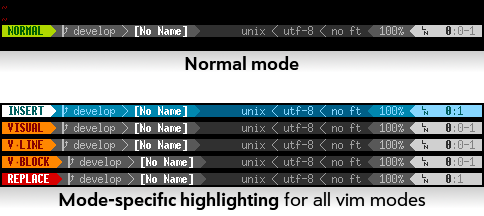
\includegraphics[scale=.4]{figures/vim_powerline_modes.png}
    \end{center}
\end{frame}


\subsection{grep}

\begin{frame}
    \frametitle{
        \href{https://github.com/vim-scripts/grep.vim}
             {grep}
    }
    \large
    Powerful integration with system's \hl{*grep} utilities, including ability
    to grep through Vim buffers \\
\end{frame}


\subsection{yankstack}

\begin{frame}
    \frametitle{
        \href{https://github.com/vim-scripts/yankstack}
             {yankstack}
    }
    Lightweight implementation of the Emacs 'kill~ring' for Vim. \\ \bigskip

    It allows you to yank and delete things without worrying about losing the
    text that you yanked previously. \\ \bigskip

    It effectively turns your default register into a stack, and lets you cycle
    through the items in the stack after doing a paste. \\
\end{frame}


\subsection{EasyMotion}

\begin{frame}
    \frametitle{
        \href{https://github.com/vim-scripts/EasyMotion}
             {EasyMotion}
    }
    \large
    Highlights all possible motion choices and allows you to press one key to
    jump directly to the target \\
\end{frame}


\subsection{MultipleSearch}

\begin{frame}
    \frametitle{
        \href{https://github.com/vim-scripts/MultipleSearch}
             {MultipleSearch}
    }
    \large
    Display multiple searches at the same time with different color highlights \\
\end{frame}


\subsection{surround}

\begin{frame}
    \frametitle{
        \href{https://github.com/vim-scripts/surround.vim}
             {surround}
    }
    \large
    Easily delete, change and add surroundings in pairs (parentheses, brackets,
    quotes, XML tags, and more) \\
\end{frame}


\subsection{repeat}

\begin{frame}
    \frametitle{
        \href{https://github.com/vim-scripts/repeat.vim}
             {repeat}
    }
    \large
    Allows to repeat complex plugin's actions
    (for example \href{https://github.com/vim-scripts/surround.vim}{surround})
    by remapping \hl{.} command \\
\end{frame}


\subsection{Align}

\begin{frame}
    \frametitle{
        \href{https://github.com/vim-scripts/Align}
             {Align}
    }
    \large
    Easily align text and program code in various ways, using multitude of
    predefined align-schemas or powerful manual control \\
\end{frame}


\subsection{DirDiff}

\begin{frame}
    \frametitle{
        \href{https://github.com/vim-scripts/DirDiff.vim}
             {DirDiff}
    }
    \large
    Performs a recursive diff on two directories and generates a diff window,
    similar to GUI diff tools like \hl{Kdiff3} or \hl{Kompare} \\
\end{frame}


\subsection{SudoEdit}

\begin{frame}
    \frametitle{
        \href{https://github.com/vim-scripts/SudoEdit.vim}
             {SudoEdit}
    }
    \large
    Allows to read/write a file from inside vim with \hl{sudo} privileges \\
\end{frame}


\subsection{gnupg}

\begin{frame}
    \frametitle{
        \href{https://github.com/vim-scripts/gnupg}
             {gnupg}
    }
    \large
    Transparent editing of \hl{gpg} encrypted files \\
\end{frame}


\subsection{file-line}

\begin{frame}
    \frametitle{
        \href{https://github.com/vim-scripts/file-line}
             {file-line}
    }
    \large
    Allows to open files as \hl{file:line} and place a cursor on chosen line \\
\end{frame}


\subsection{greplace}

\begin{frame}
    \frametitle{
        \href{https://github.com/vim-scripts/greplace.vim}
             {greplace}
    }
    \large
    Global Replace plugin allows you to search and replace a pattern across
    multiple files \\
\end{frame}


\subsection{VisIncr}

\begin{frame}
    \frametitle{
        \href{https://github.com/vim-scripts/VisIncr}
             {VisIncr}
    }
    \large
    Facilitates making a column of increasing or decreasing numbers, dates, or
    day names \\
\end{frame}


\subsection{man}

\begin{frame}
    \frametitle{man}
    \large
    Allows to read \hl{man pages} directly from vim with \hl{:Man} command \\
    \bigskip
    This plugin is part of default vim distribution and can be enabled with
    \hl{runtime! ftplugin/man.vim} command in .vimrc \\
\end{frame}


\subsection{info}

\begin{frame}
    \frametitle{
        \href{https://github.com/vim-scripts/info.vim}
             {info}
    }
    \large
    \hl{GNU info} documentation browser \\
\end{frame}


\subsection{a}

\begin{frame}
    \singleframesubtitle{Programming related plugins}
\end{frame}

\begin{frame}
    \frametitle{
        \href{https://github.com/vim-scripts/a.vim}
             {a}
    }
    \large
    Alternate between source files quickly, like \hl{.c} $\Longleftrightarrow$
    \hl{.h} etc. \\
\end{frame}


\subsection{Taglist}

\begin{frame}
    \frametitle{
        \href{https://github.com/vim-scripts/taglist.vim}
             {Taglist}
    }
    \large
    Provides an overview of the structure of source code files and allows you to
    efficiently browse through source code files for many programming languages
    \par
\end{frame}


\subsection{Tagbar}

\begin{frame}
    \frametitle{
        \href{https://github.com/vim-scripts/Tagbar}
             {Tagbar}
    }
    \large
    Similar to the \href{https://github.com/vim-scripts/taglist.vim}{Taglist}
    plugin, but is superior in some ways and provides an ability to sort
    tags by scope \\
\end{frame}


\subsection{Tagselect}

\begin{frame}
    \frametitle{
        \href{https://github.com/vim-scripts/tagselect}
             {Tagselect}
    }
    \large
    A better \hl{:tselect} and \hl{Ctrl-]} commands \\ \bigskip
    Shows matched tags in a separate window, which can be searched and scrolled
    with ordinary vim commands \\
\end{frame}


\subsection{cscope\_macros}

\begin{frame}
    \frametitle{
        \href{https://github.com/vim-scripts/cscope\_macros.vim}
             {cscope\_macros}
    }
    \large
    Handy mappings and commands to search tags with \hl{cscope} \\
\end{frame}


\subsection{fugitive}

\begin{frame}
    \frametitle{
        \href{git://github.com/tpope/vim-fugitive.git}
             {fugitive}
    }
    \large
    An awesome \hl{git} integration into vim \\
\end{frame}


\subsection{OmniCppComplete}

\begin{frame}
    \frametitle{
        \href{https://github.com/vim-scripts/OmniCppComplete}
             {OmniCppComplete}
    }
    \large
    C/C++ omni-completion with ctags database, a kind of intellisense for vim \\
\end{frame}


\subsection{clang-complete}

\begin{frame}
    \frametitle{
        \href{https://github.com/vim-scripts/clang-complete}
             {clang-complete}
    }
    \large
    Uses Clang for completing C, C++, Objective-C and Objective-C++ \\
    \bigskip
    You don't need any ctags for it to work \\
    \bigskip
    It can complete complex things, which OmniCppComplete can't \\
\end{frame}


\subsection{EnhCommentify}

\begin{frame}
    \frametitle{
        \href{https://github.com/vim-scripts/EnhCommentify.vim}
             {EnhCommentify}
    }
    \large
    Automatically comment/uncomment lines of code in various programming
    languages \\
\end{frame}


\subsection{NERDCommenter}

\begin{frame}
    \frametitle{
        \href{https://github.com/vim-scripts/The-NERD-Commenter}
             {NERDCommenter}
    }
    \large
    Another one nice commenter, it complements
    \href{https://github.com/vim-scripts/EnhCommentify.vim}{EnhCommentify},
    adding some features which the latter doesn't have \\
\end{frame}


\subsection{snipMate}

\begin{frame}
    \frametitle{
        \href{git://github.com/msanders/snipmate.vim.git}
             {snipMate}
    }
    \large
    Brings \hl{TextMate}'s snippets features in Vim for various programming
    languages \\
\end{frame}


\subsection{delimitMate}

\begin{frame}
    \frametitle{
        \href{git://github.com/Raimondi/delimitMate.git}
             {delimitMate}
    }
    \large
    Provides automatic closing of quotes, parenthesis, brackets, etc., besides
    some other related features that should make your time in insert mode a
    little bit easier \\
\end{frame}


\subsection{errormarker}

\begin{frame}
    \frametitle{
        \href{https://github.com/vim-scripts/errormarker.vim}
             {errormarker}
    }
    \large
    Highlights and sets error markers for lines with compile errors
\end{frame}


\subsection{camelcasemotion}

\begin{frame}
    \frametitle{
        \href{https://github.com/vim-scripts/camelcasemotion}
             {camelcasemotion}
    }
    \large
    Motion through \hl{CamelCaseWords} and \hl{underscore\_notation} \\
\end{frame}


\subsection{argtextobj}

\begin{frame}
    \frametitle{
        \href{http://github.com/vim-scripts/argtextobj.vim}
             {argtextobj}
    }
    \large
    Text-object like motion for function's arguments \\
\end{frame}


\subsection{BlockDiff}

\begin{frame}
    \frametitle{
        \href{http://github.com/vim-scripts/BlockDiff}
             {BlockDiff}
    }
    \large
    Shows diff between two arbitrary blocks of text \\
\end{frame}


\subsection{DoxygenToolkit}

\begin{frame}
    \frametitle{
        \href{http://github.com/vim-scripts/DoxygenToolkit.vim}
             {DoxygenToolkit}
    }
    \large
    Simplify creation of Doxygen documentation in C/C++ projects \\
\end{frame}


\subsection{Conque-Shell}

\begin{frame}
    \frametitle{
        \href{http://github.com/vim-scripts/Conque-Shell}
             {Conque-Shell}
    }
    \large
    Run interactive commands, such as \hl{bash}, inside a Vim buffer \\
\end{frame}


\subsection{Syntastic}

\begin{frame}
    \frametitle{
        \href{http://github.com/vim-scripts/Syntastic}
             {Syntastic}
    }
    \large
    It's a syntax checking plugin that runs files through external syntax
    checkers and displays any resulting errors to the user \\
    This can be done automatically or on demand \\
\end{frame}


\subsection{git\_patch\_tags}

\begin{frame}
    \frametitle{
        \href{https://github.com/vim-scripts/git\_patch\_tags.vim}
             {git\_patch\_tags}
    }
    \large
    Provides shortcuts for adding tag lines for git commits, like
    \hl{Reviewed-by:} \hl{Tested-by:} etc. with automatic user-name and email
    substitution \\
\end{frame}


\subsection{patchreview}

\begin{frame}
    \frametitle{
        \href{http://github.com/vim-scripts/patchreview.vim}
             {patchreview}
    }
    \large
    Simplify the process of reviewing multi-file patches, by showing each file
    changes in a diffsplit in separate vim tab \\
\end{frame}



\subsection{Marks-Browser}

\begin{frame}
    \singleframesubtitle{Other mics plugins}
\end{frame}

\begin{frame}
    \frametitle{
        \href{https://github.com/vim-scripts/Marks-Browser}
             {Marks-Browser}
    }
    \large
    Shows list of set marks (including special) for the current file in a
    separate window \\
\end{frame}


\subsection{ShowMarks}

\begin{frame}
    \frametitle{
        \href{https://github.com/vim-scripts/ShowMarks}
             {ShowMarks}
    }
    \large
    Visually shows the location of marks by placing a sign in the leftmost
    column of the buffer \\
\end{frame}


\subsection{diffchanges}

\begin{frame}
    \frametitle{
        \href{http://github.com/vim-scripts/diffchanges.vim}
             {diffchanges}
    }
    \large
    Show changes, made to current buffer since the last save, in a diff mode \\
\end{frame}


\subsection{xml.vim}

\begin{frame}
    \frametitle{
        \href{https://github.com/vim-scripts/xml.vim}
             {xml.vim}
    }
    \large
    Makes editing xml (and html) files a kid's play \\
\end{frame}


\subsection{DrawIt}

\begin{frame}
    \frametitle{
        \href{http://github.com/vim-scripts/DrawIt}
             {DrawIt}
    }
    \large
    Ascii drawing plugin: lines, ellipses, arrows, fills, and more \\
\end{frame}


\subsection{deb}

\begin{frame}
    \frametitle{
        \href{https://github.com/vim-scripts/deb.vim}
             {deb}
    }
    \large
    Allows to browse debian package in the same way you can browse .tar and .zip
    files \\
\end{frame}


\section{What's next}

\begin{frame}
    \singleframesubtitle{Eternal question:}
\end{frame}

\begin{frame}[plain]
    \frametitle{Vim vs Emacs}
    \begin{tikzpicture}[remember picture,overlay]
        \node[at=(current page.center), yshift=-1cm] {
            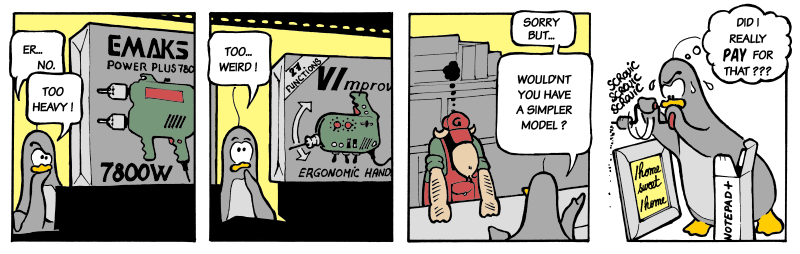
\includegraphics[width=\paperwidth]{figures/vim_vs_emacs.png}
        };
    \end{tikzpicture}
\end{frame}

\begin{frame}
    \singleframesubtitle{It doesn't matter, just choose one of them}
    \scriptsize but vim is better anyway  ; ) \\
\end{frame}

\begin{frame}[fragile]
    \frametitle{Give it a try \hl{;)}}

    \large
    Check out my \href{https://github.com/chumakd/vim-runtime/blob/master/vimrc}{.vimrc}
    config on \href{https://github.com/chumakd/vim-runtime}{github} \\ \bigskip

    To try my vim configuration just do the following: \\ \bigskip

    \smallskip
    \scriptsize
    \verb|$ git clone git://github.com/chumakd/vim-runtime.git| \\ \smallskip
    \verb|$ cd vim-runtime| \\ \smallskip
    \verb|$ git submodule update --init| \\ \smallskip
    \verb|$ cd ..| \\ \smallskip
    \verb|$ MYVIMRC=./vim-runtime/vimrc VIMHOME=./vim-runtime \| \\
    \verb|  gvim ./vim-runtime/vimrc| \\
\end{frame}

\begin{frame}
    \begin{center}
        \titlefontsize F!N
    \end{center}
\end{frame}


\end{document}
